\section{WKB aproximace}

\begin{theory}
	WKB\footnote{
    Metodu rozpracovali fyzici Gregor Wentzel, Hendrik Kramers, Léon Brillouin (1926) a paralelně matematik Harold Jeffreys (1923), někdy se proto též nazývá JWKB nebo WKBJ metoda.
    Poprvé ji však popsali o století dříve Joseph Liouville a George Green (1837) a v některých zdrojích se tudíž uvádí jako LG metoda.
    Přínos autorů WKBJ byl v zavedení navazovacích podmínek v bodech obratu.
}\index{aproximace!WKB}
je kvaziklasická aproximace jednorozměrné Schrödingerovy rovnice
\begin{equation}
    -\frac{\hbar^{2}}{2M}\psi''(x)+V(x)\psi(x)=E\psi(x).
\end{equation}
Rovnice se přepíše do tvaru
\begin{equation}
    \label{eq:WKBSchrodingerp}
    \psi''(x)=-\frac{p^{2}}{\hbar^{2}}\psi(x),
\end{equation}
kde
\begin{equation}
    p=\pm\sqrt{2M\left[E-V(x)\right]}
\end{equation}
je klasická hybnost částice.
Vlnová funkce se následně hledá ve tvaru
\begin{equation}
    \psi(x)=A(x)\e^{\frac{\im}{\hbar}S(x)},
\end{equation}
kde obě funkce $A(x), S(x)$ jsou reálné; udávají tedy amplitudu a fázi.
Dosazení do Schrödingerovy rovnice~\eqref{eq:WKBSchrodingerp} vede na dvě rovnice (jednu pro reálnou a druhou pro imaginární část)
\begin{subequations}
    \begin{align}
        \hbar^{2}\frac{A''(x)}{A(x)}-\left[S'(x)\right]^{2}&=-p^{2},\\
        2A'(x)S'(x)+A(x)S''(x)&=0.
    \end{align}        
\end{subequations}
Řešení druhé rovnice je 
\begin{align}
    \left[A^{2}(x)S'(x)\right]'&=0 && \Longrightarrow & A(x)&=\frac{C}{S'(x)}.
\end{align}
V první rovnici se zanedbá člen $\hbar^{2}$ a navíc se předpokládá, že \uv{oscilace} amplitudy $A(x)$ jsou mnohem menší než amplituda sama.
Tím se rovnice zjednoduší a funkci $S(x)$ lze nalézt integrováním
\begin{align}
    \left[S'(x)\right]^{2}&=p^{2} && \Longrightarrow & S'(x)&=\pm\abs{p(x)} && \Longrightarrow & S(x)=\pm\int_{x_{0}}^{x}\abs{p(x')}\d x',
\end{align}
což je výraz pro klasickou akci.\index{akce!klasická}

WKB vlnová funkce má tedy tvar
\begin{equation}
    \psi(x)=\frac{1}{\sqrt{\abs{p(x)}}}\left[C\e^{\frac{\im}{\hbar}\int_{x_{0}}^{x}\abs{p(x')}\d x'}+D\e^{-\frac{\im}{\hbar}\int_{x_{0}}^{x}\abs{p(x')}\d x'}\right],
\end{equation}
kde $x_{0}$ je libovolný bod, od kterého se integruje, a $C,D$ jsou normalizační konstanty (změna integrační meze $x_0$ pouze změní celkovou fázi vlnové funkce).

V kinematicky nedostupné oblasti, ve které je $E<V(x)$, vlnová funkce přejde od oscilujícího řešení k~exponenciálně ubývajícím řešením
\begin{equation}
    \psi(x)=\frac{1}{\sqrt{\abs{p(x)}}}\left[E\e^{\frac{1}{\hbar}\int_{x_{0}}^{x}\abs{p(x')}\d x'}+F\e^{-\frac{1}{\hbar}\int_{x_{0}}^{x}\abs{p(x')}\d x'}\right].
\end{equation}
	\sec{Lineární navazovací podmínky}\index{vlnová funkce!sešívání}
V bodech obratu $p(x_{1,2})=0$,\index{bod!obratu} které ohraničují kinematicky dostupnou oblast, vlnová funkce WKB aproximace diverguje.
Vlnová funkce je přitom nenulová vně i uvnitř kinematicky dostupné oblasti, a je proto nutné ji přes bod obratu správně navázat.
To lze provést buď přes komplexní rozšíření souřadnice~\cite{Cejnar2013}, nebo přes aproximaci potenciálu v okolí bodu obratu. 
Pokud $p'(x_{1,2})\neq0$ a zároveň $p'(x)$ je spojitá v bodech $x_{1,2}$, pak se potenciál v okolí bodů obratu aproximuje lineární funkcí, pro kterou je známo přesné řešení Schrödingerovy rovnice ve tvaru Airyho funkcí~\cite{Formanek2004}.\index{funkce!Airyho}

\begin{figure}[!htbp]
    \begin{subfigure}{0.45\linewidth}
        \centering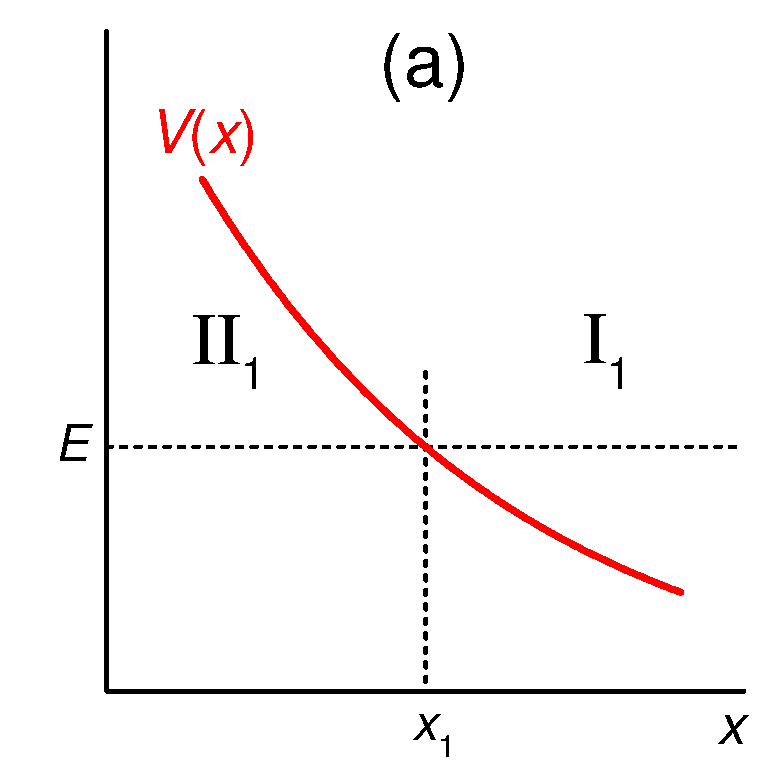
\epsfig{file=wkb_down.eps,width=\linewidth}
    \end{subfigure}
    \hfill
    \begin{subfigure}{0.45\linewidth}
        \centering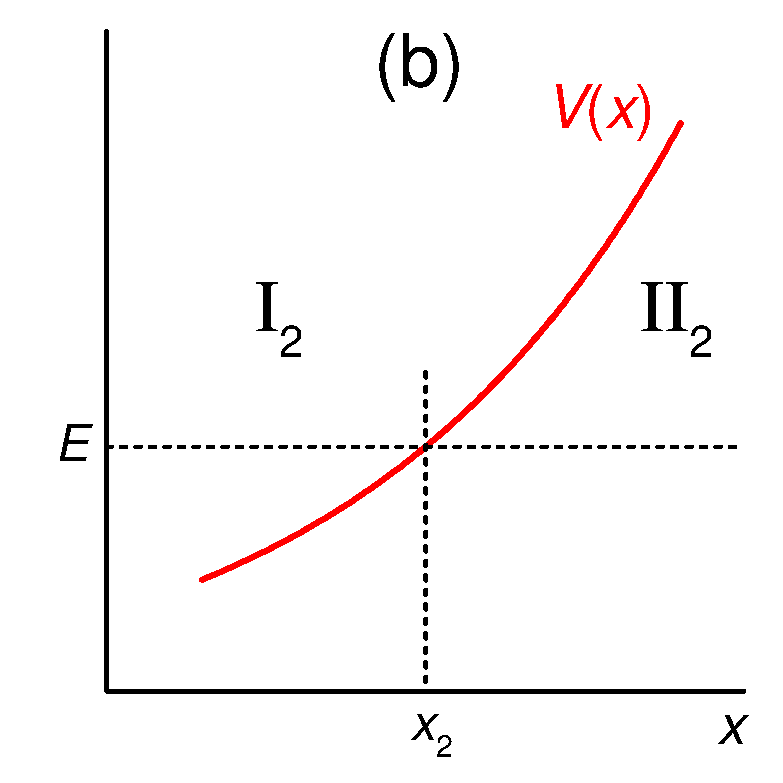
\epsfig{file=wkb_up.eps,width=\linewidth}	
    \end{subfigure}
    \scaption{
        Body obratu pro navazování WKB vlnových funkcí.
    }
\label{fig:WKBConnection}
\end{figure}				

\begin{itemize}
\item
    V bodě obratu $x_{1}$, ve kterém potenciál klesá, $V'(x_{1})<0$, viz obrázek~\ref{fig:WKBConnection}(a), se mění fáze vlnové funkce o $\frac{\pi}{4}$ a zdvojnásobuje se amplituda u sinové části:
    \begin{subequations}
        \begin{align}
            \psi_{\mathrm{II}_{1}}(x)&=\frac{C_{1}}{\sqrt{\abs{p(x)}}}\e^{-\frac{1}{\hbar}\int_{x}^{x_{1}}\abs{p(x')}\d x'},\\
            \psi_{\mathrm{I}_{1}}(x)&=\frac{2C_{1}}{\sqrt{\abs{p(x)}}}\sin\left[\frac{1}{\hbar}\int_{x_{1}}^{x}p(x')\d x'+\frac{\pi}{4}\right]
        \end{align}            
        \label{eq:WKBConnectionDown1}
    \end{subequations}
    a
    \begin{subequations}
        \begin{align}
            \psi_{\mathrm{II}_{1}}(x)&=\frac{C_{1}}{\sqrt{\abs{p(x)}}}\e^{\frac{1}{\hbar}\int_{x}^{x_{1}}\abs{p(x')}\d x'},\\
            \psi_{\mathrm{I}_{1}}(x)&=\frac{C_{1}}{\sqrt{\abs{p(x)}}}\cos\left[\frac{1}{\hbar}\int_{x_{1}}^{x}p(x')\d x'+\frac{\pi}{4}\right],
        \end{align}		            
        \label{eq:WKBConnectionDown2}
    \end{subequations}
    kde oblast II$_{1}$ odpovídá $x<x_{1}$ a oblast I$_{1}$ odpovídá $x>x_{1}$.
    Integrační meze v integrálech jsou zvoleny tak, aby spodní mez byla vždy menší než horní mez, a tedy integrace probíhala postupně zleva doprava.
    
\item
    V bodě obratu $x_{2}$, ve kterém potenciál roste, $V'(x_{2})>0$, viz obrázek~\ref{fig:WKBConnection}(b), je analogicky\footnote{
        Navazovací podmínky~\eqref{eq:WKBConnectionUp1}--\eqref{eq:WKBConnectionUp2} jsou samozřejmě zcela ekvivalentní podmínkám~\eqref{eq:WKBConnectionDown1}--\eqref{eq:WKBConnectionDown2} a zde jsou vypsány jen pro úplnost a pro rychlejší referenci v příkladech.
    }
    \begin{subequations}
        \begin{align}
            \psi_{\mathrm{I}_{2}}(x)&=\frac{2C_{2}}{\sqrt{\abs{p(x)}}}\sin\left[\frac{1}{\hbar}\int_{x}^{x_{2}}p(x')\d x'+\frac{\pi}{4}\right],\\
            \psi_{\mathrm{II}_{2}}(x)&=\frac{C_{2}}{\sqrt{\abs{p(x)}}}\e^{-\frac{1}{\hbar}\int_{x_{2}}^{x}\abs{p(x')}\d x'}\,,
        \end{align}            
        \label{eq:WKBConnectionUp1}
    \end{subequations}
    nebo
    \begin{subequations}
        \begin{align}
            \psi_{\mathrm{I}_{2}}(x)&=\frac{C_{2}}{\sqrt{\abs{p(x)}}}\cos\left[\frac{1}{\hbar}\int_{x}^{x_{2}}p(x')\d x'+\frac{\pi}{4}\right],\\
            \psi_{\mathrm{II}_{2}}(x)&=\frac{C_{2}}{\sqrt{\abs{p(x)}}}\e^{\frac{1}{\hbar}\int_{x_{2}}^{x}\abs{p(x')}\d x'},
        \end{align}            
        \label{eq:WKBConnectionUp2}
    \end{subequations}
    kde oblast I$_{2}$ odpovídá $x<x_{2}$ a oblast II$_{2}$ odpovídá $x>x_{2}$.
\end{itemize}

\sec{Kvadratické navazovací podmínky}
	V případě kvadratické bariéry lze navazující podmínky před a po bariéře vyjádřit například v tomto tvaru:
    \begin{subequations}
        \begin{align}
            \psi_{\mathrm{I}}(x)
                &=C\frac{\e^{-\pi\epsilon}}{\sqrt{p(x)}}
                \e^{\pm\frac{\im}{\hbar}\int_{x}^{a}p(x')\d x'\mp\im\frac{\pi}{4}}
                +C\frac{\sqrt{1+\e^{-2\pi\epsilon}}}{\sqrt{p(x)}}
                \e^{\mp\frac{\im}{\hbar}\int_{x}^{a}p(x')\d x'\pm\im\frac{\pi}{4}}\e^{\pm\im\phi(\epsilon)},
            \psi_{\mathrm{II}}(x)
                &=\frac{C}{\sqrt{p(x)}}
                \e^{\pm\frac{\im}{\hbar}\int_{b}^{x}p(x')\d x'\pm\im\frac{\pi}{4}},
        \end{align}            
    \end{subequations}
	přičemž v případě horních znamének odpovídá první vlna odražené vlně, druhá vlna dopadající vlně a třetí vlna prošlé vlně.
	Dodatečný fázový posun má vyjádření
	\begin{equation}
		\phi(\epsilon)=\epsilon+\arg\Gamma\left(\frac{1}{2}+\im\epsilon\right)-\epsilon\ln\abs{\epsilon}.
	\end{equation}
	Uvedený vztah platí pod i nad bariérou, kdy se do integrálů akce dosadí $c$ namísto $a$ a $b$.
    
	\sec{Bohrovo-Sommerfeldovo kvantování}\index{kvantování!Bohrovo-Sommerfeldovo}
Omezme se nyní na vázané stavy, tj. na stavy, jejichž vlnová funkce $\psi(x\pm\infty)=0$.
Vyskytují-li se na zadané energii jen dva body obratu, pak musí platit $\psi_{\mathrm{I}_{1}}(x)=\psi_{\mathrm{I}_{2}}(x)$, což je splněno, pokud
\begin{itemize}
\item
    $C_{1}=C_{2}$ a zároveň
    \begin{equation}
        \sin\left[\frac{1}{\hbar}\int_{x_{1}}^{x}p(x')\d x'+\frac{\pi}{4}\right]=\sin\left[\frac{1}{\hbar}\int_{x}^{x_{2}}p(x')\d x'+\frac{\pi}{4}\right],
    \end{equation}
    neboli
    \begin{equation}
        \frac{1}{\hbar}\int_{x_{1}}^{x}p(x')\d x'+\frac{\pi}{4}+n\pi=\frac{1}{\hbar}\int_{x}^{x_{2}}p(x')\d x'+\frac{\pi}{4},
    \end{equation}
    nebo vhodněji pokud	
\item
    $C_{1}=-C_{2}$ a zároveň
    \begin{equation}
        \sin\left[\frac{1}{\hbar}\int_{x_{1}}^{x}p(x')\d x'+\frac{\pi}{4}\right]=-\sin\left[\frac{1}{\hbar}\int_{x}^{x_{2}}p(x')\d x'+\frac{\pi}{4}\right],
    \end{equation}
    neboli
    \begin{equation}
        \frac{1}{\hbar}\int_{x_{1}}^{x}p(x')\d x'+\frac{\pi}{4}+n\pi=-\frac{1}{\hbar}\int_{x}^{x_{2}}p(x')\d x'-\frac{\pi}{4}.
    \end{equation}
\end{itemize}
Z poslední rovnosti plyne \emph{Bohrova-Sommerfeldova kvantovací podmínka}
\begin{equation}
    \label{eq:BohrSommerfeld}
    \important{\oint p(x')\d x'=2\int_{x_{1}}^{x_{2}}p(x')\d x'=2\pi\hbar\left(n+\frac{1}{2}\right)},
\end{equation}
kde $n\in\mathbb{N}_{0}$.	
Tento výraz platí jen pro \uv{měkké} body obratu.
Za každý \uv{tvrdý} bod obratu (odraz o nekonečně vysokou bariéru) je nutné do závorky přidat ještě $\frac{1}{4}$.

        
    \begin{note}[Značení:]
        Pro zjednodušení notace se v následujícím textu budou využívat substituce
		\begin{subequations}
			\begin{align}
				\lambda(x)&\equiv\frac{C}{\sqrt{\abs{p(x)}}},\\
				S_{a}^{b}&\equiv\frac{1}{\hbar}\int_{a}^{b}\abs{p(x')}\d x'.
				\label{eq:WKBNotation}
			\end{align}					
		\end{subequations}
        Navazovací podmínky~\eqref{eq:WKBConnectionDown1} se pak kompaktně zapíší jako
		\begin{subequations}
			\begin{align}
				\psi_{\mathrm{II}_{1}}(x)&=\lambda(x)\e^{-S_{x}^{x_{1}}},\\
				\psi_{\mathrm{I}_{1}}(x)&=2\lambda(x)\sin\left[S_{x_{1}}^{x}+\frac{\pi}{4}\right].
			\end{align}				
		\end{subequations}
    \end{note}
\end{theory}

\subsection{Nekonečně hluboká pravoúhlá jáma se schodem}   
Částice o hmotnosti $M$ se pohybuje v potenciálu
\begin{equation}
    V(x)=\left\{\begin{array}{ll} \infty & x<0 \\ V_{0} & 0<x<\frac{a}{2} \\ 0 & \frac{a}{2}<x<a \\ \infty & x>a\end{array}\right.
\end{equation}
viz obrázek~\ref{fig:WKBStep}.
Nalezněte WKB vlnovou funkci a spektrum pro $E>V_{0}$.

\begin{figure}[!htbp]
	\centering
		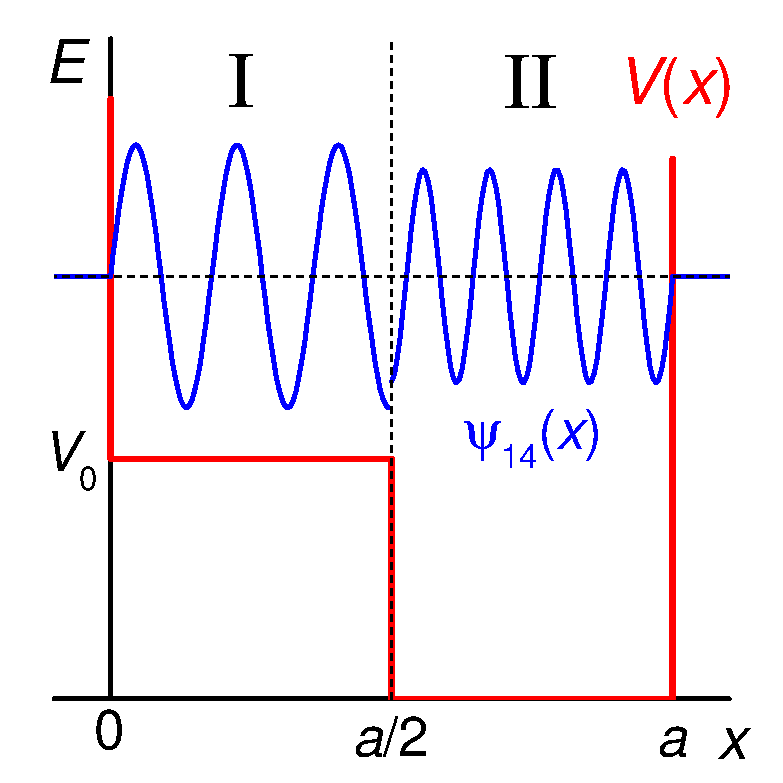
\epsfig{file=schod.eps,width=0.4\linewidth,keepaspectratio}
		\scaption{
			Nekonečně hluboká pravoúhlá jáma se schodem.
			Potenciál červeně.
			Modře zobrazena 14. vlnová funkce pro hodnoty parametrů $a=V_{0}=2$, $M=1$, $\hbar=0.1$.
			Příslušná energie je $E_{14}=3,52$.
		}
	\label{fig:WKBStep}
\end{figure}		
	
\begin{solution}
	Kinematicky dostupné oblasti označíme
	\begin{align}
		\text{I:} & \quad 0<x<\frac{a}{2}\,, \nonumber\\
		\text{II:} & \quad \frac{a}{2}<x<a\,.\nonumber
	\end{align}
	Klasická hybnost v těchto oblastech pak je
    \begin{subequations}
        \begin{align}
            p_{\mathrm{I}}&=\sqrt{2M\left(E-V_{0}\right)},\\
            p_{\mathrm{II}}&=\sqrt{2ME}
        \end{align}            
    \end{subequations}
	(hybnost je v uvedených intervalech konstantní, nezávisí na souřadnici).
	Zintegrování v mezích $(0,x)$ dá akci
    \begin{subequations}
        \begin{align}
            S_{\mathrm{I}}(x)&=\int_{0}^{x}p_{\mathrm{I}}\d x'=xp_{\mathrm{I}},\\
            S_{\mathrm{II}}(x)
                &=\int_{0}^{\frac{a}{2}}p_{\mathrm{I}}\d x'+\int_{\frac{a}{2}}^{x}p_{\mathrm{II}}\d x'=\frac{a}{2}p_{\mathrm{I}}+\left(x-\frac{a}{2}\right)p_{\mathrm{II}}.
        \end{align}            
    \end{subequations}
	Vlnová funkce tedy je
    \begin{subequations}
        \begin{align}
            \psi_{\mathrm{I}}(x)&=\frac{1}{\sqrt{\abs{p_{\mathrm{I}}}}}\left[C\sin{\frac{S_{\mathrm{I}}(x)}{\hbar}}+D\cos{\frac{S_{\mathrm{I}}(x)}{\hbar}}\right],\\
            \psi_{\mathrm{II}}(x)&=\frac{1}{\sqrt{\abs{p_{\mathrm{II}}}}}\left[C\sin{\frac{S_{\mathrm{II}}(x)}{\hbar}}+D\cos{\frac{S_{\mathrm{II}}(x)}{\hbar}}\right]
        \end{align}            
    \end{subequations}
	(komplexní exponenciály byly rozepsány pomocí funkcí $\sin$, $\cos$).
	Díky tomu, že se obě akce počítají od stejného počátečního bodu $x_{0}=0$, jsou konstanty $C,D$ pro vlnové funkce v obou oblastech stejné.
	
	V dalším kroku se aplikují okrajové podmínky:
	\begin{subequations}
		\begin{align}
			\psi_{\mathrm{I}}(0)&=0 && \Longrightarrow & D&=0,\\
			\psi_{\mathrm{II}}(a)&=0 && \Longrightarrow & \sin{\frac{S_{\mathrm{II}}(x)}{\hbar}}&=0.
		\end{align}			
	\end{subequations}
	Z druhé rovnice vyplývá postupně
	\begin{align}
		S_{\mathrm{II}}(x)&=\pi n\nonumber\\
		\frac{a}{2\hbar}\left[\sqrt{2M(E-V_{0})}+\sqrt{2ME}\right]&=\pi n\nonumber\\
		E-\frac{V_{0}}{2}+\sqrt{E(E-V_{0})}&=2\underbrace{\frac{\pi^{2}\hbar^{2}n^{2}}{2Ma^{2}}}_{E_{n}^{(0)}}\nonumber\\
		E_{n}^{(0)}-E+\frac{V_{0}}{2}&=\sqrt{E(E-V_{0})}\nonumber\\
		E_{n}\equiv E&=E_{n}^{(0)}+\frac{V_{0}}{2}+\frac{V_{0}^{2}}{16E_{n}^{(0)}}\,,
		\label{eq:WKBStepEnergy}
	\end{align}
	kde $E_{n}^{(0)}$, $n\in\mathbb{N}$ označuje $n$-tou hladinu nekonečně hluboké pravoúhlé jámy.
	Pro energie dostatečně vysoko nad $V_{0}$ vymizí poslední člen, což znamená, že částice se pohybuje, jako kdyby se schod rozprostřel po celé šířce jámy a dno jámy se tak zvedlo o $V_{0}/2$.

	Explicitně vyjádřená vlnová funkce je
	\begin{subequations}
		\begin{align}
			\psi_{\mathrm{I},n}(x)&=\frac{c}{\sqrt[4]{2M\left(E_{n}-V_{0}\right)}}\sin{\left\{\frac{\sqrt{2M\left(E_{n}-V_{0}\right)}}{\hbar}x\right\}},\\
			\psi_{\mathrm{II},n}(x)&=\frac{c}{\sqrt[4]{2ME_{n}}}\sin{\left\{\frac{\sqrt{2M\left(E_{n}-V_{0}\right)}}{\hbar}\frac{a}{2}+\frac{\sqrt{2ME_{n}}}{\hbar}\left(x-\frac{1}{2}\right)\right\}}\,,
		\end{align}			
	\end{subequations}
	kde energie jsou dány vzorcem~\eqref{eq:WKBStepEnergy}.
	
	WKB vlnová funkce \emph{není spojitá} v bodě $x=\frac{a}{2}$, což je patrné z příkladu na obrázku~\ref{fig:WKBStep}.
\end{solution}

\subsection{Harmonický oscilátor}
	\begin{enumerate}
		\item
			Použitím WKB metody nalezněte spektrum a odpovídající vlnové funkce jednorozměrného harmonického oscilátoru
			popsaného (již známým) Hamiltoniánem
			\begin{equation}
			\operator{H}
				=\frac{1}{2M}\operator{p}^{2}+\frac{1}{2}M\Omega^{2}\operator{x}^{2}
			\end{equation}
			($M$ je hmotnost částice, která se v potenciálu pohybuje, $\Omega$ úhlová frekvence kmitů).
		
		\item
			Nakreslete graf vlnové funkce pro dvacátou energetickou hladinu ($n=20$) a porovnejte s přesnou vlnovou funkcí, která je řešením Schrödingerovy rovnice a která je
			určena Hermitovými polynomy
			\begin{equation}
			\phi_{n}(x)
				=\sqrt[4]{\frac{M\Omega}{\pi\hbar}}\frac{1}{\sqrt{n!2^{n}}}\,
					H_{n}(\xi)\,\e^{-\xi^{2}},\quad\xi=\sqrt{\frac{M\Omega}{\hbar}}x.
			\end{equation}
		
		\item
			Na základě tohoto srovnání diskutujte přesnost WKB metody.
	\end{enumerate}

\begin{solution}
	\begin{figure}[!htbp]
	\centering
	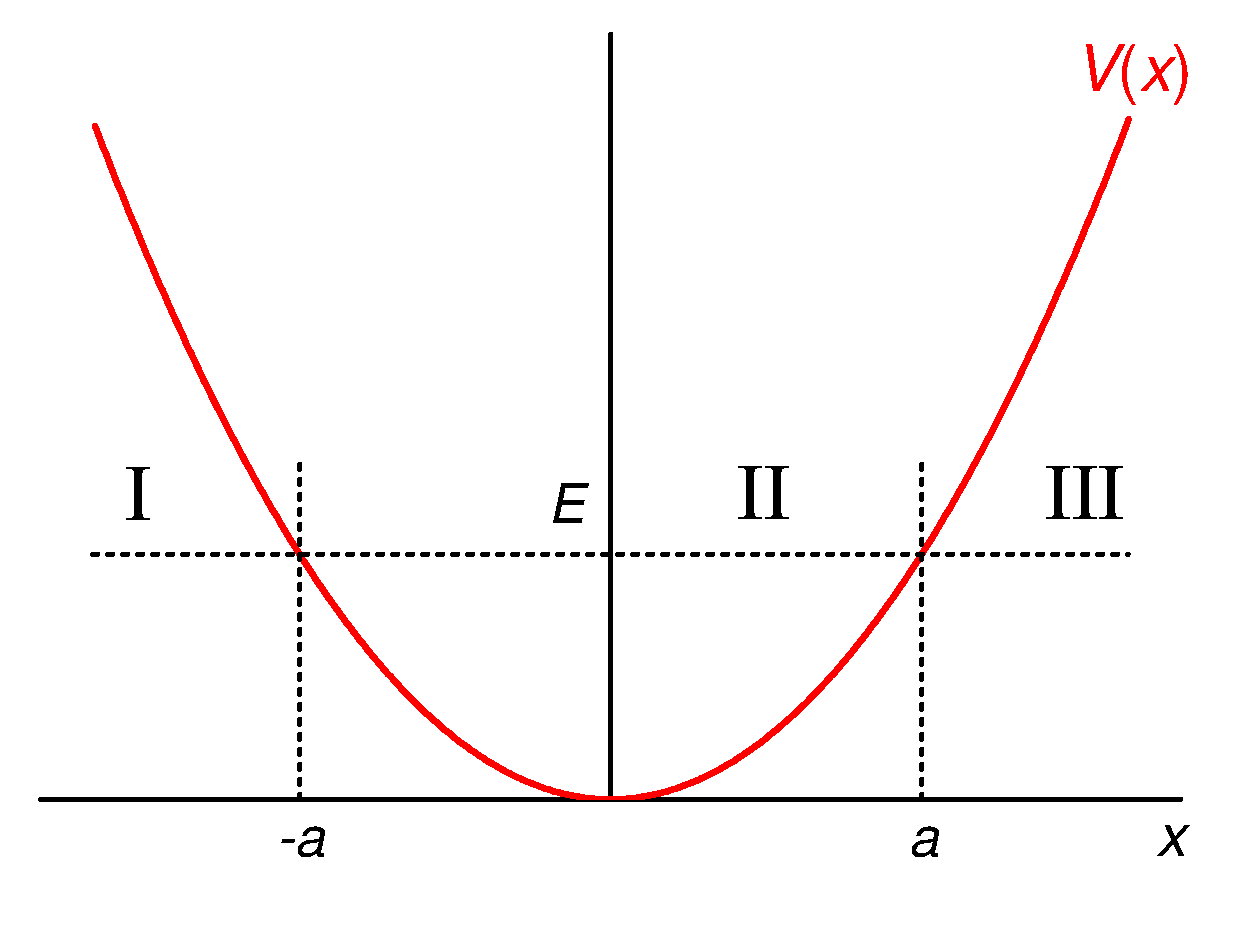
\epsfig{file=figures/ho.eps,width=0.6\linewidth,keepaspectratio}
	\caption{
		Potenciál harmonického oscilátoru s vyznačenými oblastmi pro WKB řešení.
	}
	\label{fig:WKBHarmonicOscillator}
	\end{figure}	
		
	Potenciál harmonického oscilátoru je znázorněn na obrázku~\ref{fig:WKBHarmonicOscillator}.
	Body obratu jsou $\pm a$, kde
	\begin{equation}
		a=\sqrt{\frac{2E}{M\Omega^{2}}}.
	\end{equation}
	Vlnová funkce v oblasti I (III) musí být WKB vlna, která ubývá pro $x\rightarrow-\infty$ ($x\rightarrow\infty$), takže
	\begin{subequations}
		\begin{align}
			\psi_{\mathrm{I}}(x)&=\frac{C}{\sqrt{\abs{p(x)}}}\e^{-\frac{1}{\hbar}\int_{x}^{-a}\abs{p(x')}\d x'}\equiv\lambda\e^{-I_{x}^{-a}},\\
			\psi_{\mathrm{III}}(x)&=\lambda'\e^{-I_{a}^{x}},
		\end{align}				
	\end{subequations}
	kde jsme použili značení~\eqref{eq:WKBNotation}.
	Klasická hybnost je
	\begin{equation}
		p(x)=\sqrt{2M\left(E-\frac{1}{2}M\Omega^{2}x^{2}\right)}.
	\end{equation}	
	Pomocí sešívacích vztahů~\eqref{eq:WKBConnectionDown1} se napojí vlnová funkce v oblasti II:
	\begin{equation}
		\psi_{\mathrm{II}}(x)=2\lambda\sin{\left[I_{-a}^{x}+\frac{\pi}{4}\right]}=2\lambda'\sin{\left[I_{x}^{a}+\frac{\pi}{4}\right]}.
	\end{equation}
	Vychází tedy $\lambda=-\lambda'$ a
	\begin{equation}
		\label{eq:WKBHarmonicOscillatorBS}
		I_{-a}^{a}=\pi\left(n+\frac{1}{2}\right),
	\end{equation}
	což je Bohrova-Sommerfeldova kvantovací podmínka.
	
	Zbývá spočítat integrál
	\begin{align}
		I_{x_{1}}^{x_{2}}
			&=\frac{1}{\hbar}\int_{x_{1}}^{x_{2}}p(x)\d x=\frac{1}{\hbar}\int_{x_{1}}^{x_{2}}\sqrt{2M\left(E-\frac{1}{2}M\Omega^{2}x^{2}\right)}\nonumber\\
			&=\frac{\sqrt{2ME}}{\hbar}\int_{x_{1}}^{x_{2}}\sqrt{1-\underbrace{\frac{M\Omega^{2}}{2E}}_{\frac{1}{a^{2}}}x^{2}}\,\d x=\equationcomment{y=\frac{x}{a} \\ \d x=a\d y}\nonumber\\
			&=\frac{2E}{\hbar\Omega}\int_{\frac{x_{1}}{a}}^{\frac{x_{2}}{a}}\sqrt{1-y^{2}}\,\d y,
	\end{align}
	přičemž primitivní funkce k poslednímu integrálu je
	\begin{align}
		\int\sqrt{1-y^{2}}\,\d y
			&=\equationcomment{y=\sin{z} \\ \d y=\cos{z} \d z}=\int\sqrt{1-\sin^{2}z}\,\cos{z}\,\d z\nonumber\\
			&=\int\cos^{2}\,\d z=\int\frac{1+\cos{2z}}{2}\d z=\frac{1}{2}\left(z+\frac{1}{2}\sin{2z}\right)\nonumber\\
			&=\frac{1}{2}\left(z+\sin{z}\cos{z}\right)=\frac{1}{2}\left(\arcsin{y}+y\sqrt{1-y^{2}}\right),
			\label{eq:intsqrt}
	\end{align}
	takže
	\begin{equation}
		I_{x_{1}}^{x_{2}}=\frac{E}{\hbar\Omega}\left[\arcsin{y}+y\sqrt{1-y^{2}}\right]_{\frac{x_{1}}{a}}^{\frac{x_{2}}{a}}.
	\end{equation}
	Po dosazení vyjádření tohoto integrálu do kvantovacích podmínek~\eqref{eq:WKBHarmonicOscillatorBS} vychází
	\begin{align}
		I_{-a}^{a}&=\frac{E}{\hbar\Omega}\pi=\pi\left(n+\frac{1}{2}\right) && \Longrightarrow & E_{n}=\hbar\Omega\left(n+\frac{1}{2}\right),
	\end{align}
	což je přesné spektrum harmonického oscilátoru.

	Zbývá určit ještě vlnové funkce.
	V oblasti II je
	\begin{align}
		\psi_{\mathrm{II}}(x)
			&=2\lambda\sin{\left\{\frac{E}{\hbar\Omega}\left[\arcsin{y}+y\sqrt{1-y^{2}}\right]_{\frac{x}{a}}^{\frac{a}{a}=1}+\frac{\pi}{4}\right\}}\nonumber\\
			&=2\lambda\sin{\left[\frac{E}{\hbar\Omega}\left(\underbrace{\frac{\pi}{2}-\arcsin{\frac{x}{a}}}_{\arccos{\frac{x}{a}}}-\frac{x}{a}\sqrt{1-\frac{x^{2}}{a^{2}}}\right)+\frac{\pi}{4}\right]}\nonumber\\
			&=\frac{2C}{\sqrt{p(x)}}\sin\left[\frac{E}{\hbar\Omega}\left(\arccos{\frac{x}{a}}-\frac{x}{a}\sqrt{1-\frac{x^{2}}{a^{2}}}\right)+\frac{\pi}{4}\right].
	\end{align}
	
	V klasicky zakázaných oblastech I a III vychází integrál
	\begin{align}
		I_{x_{1}}^{x_{2}}
			&=\frac{2E}{\hbar\Omega}\int_{\frac{x_{1}}{a}}^{\frac{x_{2}}{a}}\sqrt{y^{2}-1}\,\d y
			 =\frac{E}{\hbar\Omega}\left[-\arccosh{y}+y\sqrt{y^{2}-1}\right]_{\frac{x_{1}}{a}}^{\frac{x_{2}}{a}}\nonumber\\
			&=\frac{E}{\hbar\Omega}\left[-\ln{\left(y+\sqrt{y^{2}-1}\right)}+y\sqrt{y^{2}-1}\right]_{\frac{x_{1}}{a}}^{\frac{x_{2}}{a}},
	\end{align}
	takže	
	\begin{align}
		\psi_{\mathrm{I}}(x)
			&=(-1)^{n}\lambda\exp\left\{-\frac{E}{\hbar\Omega}\left[-\underbrace{\ln{\left(y+\sqrt{y^{2}-1}\right)}}_{\ln(-z)=\ln{\abs{z}}+\im\pi}+y\sqrt{y^{2}-1}\right]_{\frac{x}{a}}^{-1}\right\}\nonumber\\
			&=(-1)^{n}\frac{C}{\sqrt{\abs{p(x)}}}\e^{\frac{E}{\hbar\Omega}\left[\ln{\left(-\frac{x}{a}+\sqrt{\frac{x^{2}}{a^{2}}-1}\right)}+\frac{x}{a}\sqrt{\frac{x^{2}}{a^{2}}-1}\right]}
	\end{align}
	a
	\begin{align}
		\psi_{\mathrm{III}}(x)
			&=\lambda\e^{-\frac{E}{\hbar\Omega}\left[-\arccosh{y}+x\sqrt{y^{2}-1}\right]_{1}^{\frac{x}{a}}}
			 =\frac{C}{\sqrt{\abs{p(x)}}}\e^{-\frac{E}{\hbar\Omega}\left[-\arccosh{\frac{x}{a}}+\frac{x}{a}\sqrt{\frac{x^{2}}{a^{2}}-1}\right]}.
	\end{align}
	Konstanta $C$ se určí z normalizace, přičemž pro $n$ velké a $\hbar=\Omega=M=1$ konverguje k hodnotě $C\rightarrow1/\sqrt{2\pi}$.
	
	\begin{figure}[!htbp]
		\centering
		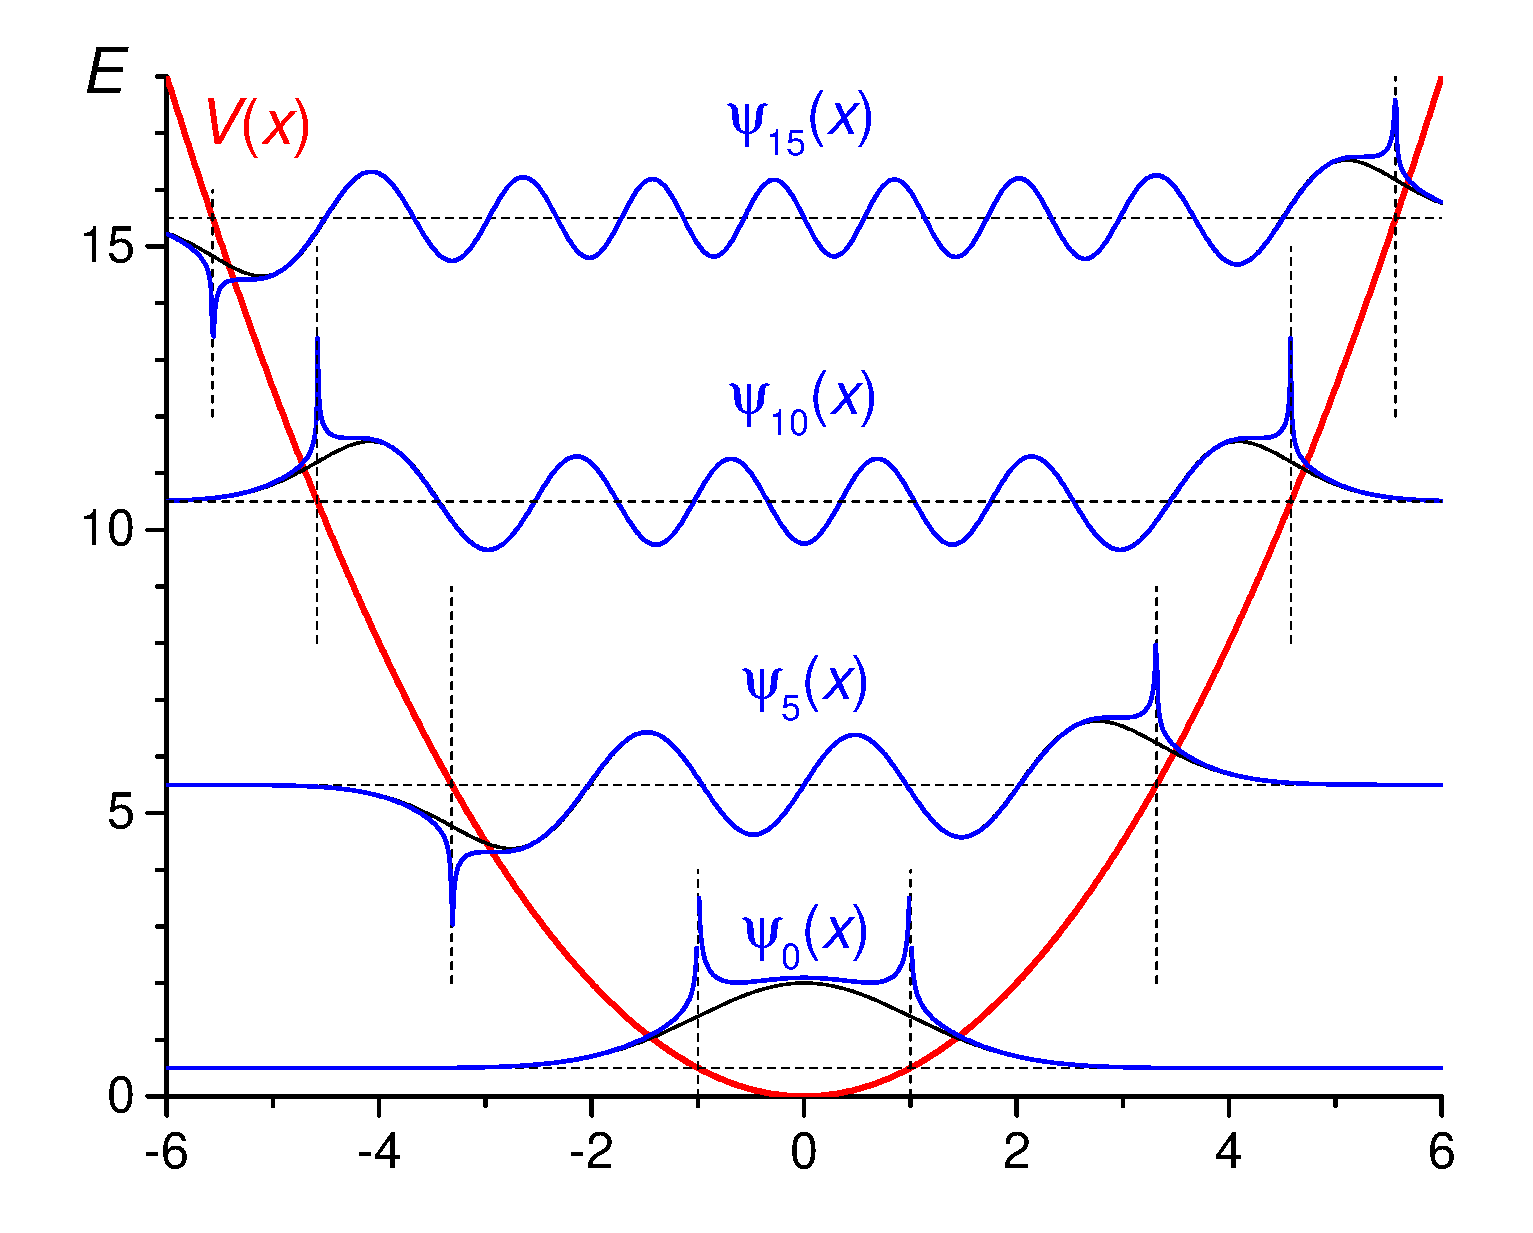
\epsfig{file=figures/howf.eps,width=0.7\linewidth,keepaspectratio}
		\scaption{
			Vlnové funkce harmonického oscilátoru s $\Omega=M=\hbar=1$ pro energie $E_{0}=\frac{1}{2}$, $E_{5}=\frac{11}{2}$, $E_{10}=\frac{21}{2}$, $E_{15}=\frac{31}{2}$.
			Přesné vlnové funkce dané Hermitovými polynomy jsou zobrazeny černými plnými čarami, odpovídající WKB aproximace jsou zobrazeny modrými plnými čarami
			(WKB vlnové funkce divergují v klasických bodech obratu, tj. v bodech, kde $E_{n}=V(x)$).
			WKB vlnové funkce jsou normalizované faktorem $1/\sqrt{2\pi}$.
		}
		\label{fig:howf}
	\end{figure}	
	
	Několik vlnových funkcí je znázorněno na obrázku~\ref{fig:howf}.
	Je vidět, že kromě bodu obratu WKB vlnová funkce velmi přesně aproximuje přesnou vlnovou funkci harmonickému oscilátoru.
\end{solution}
\subsection{$\alpha$ rozpad}
	Rozpad $\alpha$, například rozpad radia na radon\footnote{
		Použitá notace je ${}^{A}_{Z}\mathrm{X}$, kde $A=N+Z$ je celkový počet nukeonů nuklidu $\mathrm{X}$, $N$ je počet neutronů a $Z$ počet protonů = náboj jádra.
	}
	\begin{equation}
		{}^{224}_{\ 88}\mathrm{Ra}\stackrel{T_{1/2}=3.6\text{ dní}}{\longrightarrow}{}^{220}_{\ 86}\mathrm{Rn}+{}^{4}_{2}\mathrm{He}
	\end{equation}
	lze popsat modelem založeným na WKB aproximaci, který i přes svoji jednoduchost dává předpovědi, které kvalitativně souhlasí s experimentem.
	Představme si, že $\alpha$ částice vázaná v jádře tuneluje Coulombickou bariérou.
	Celý problém popíšeme jednorozměrným potenciálem (viz obrázek~\ref{fig:AlphaDecay})
	\begin{equation}
		V(x)=
			\begin{cases}
				-V_{0} & \text{pro }\abs{x}<a \\
				\frac{Z_{\alpha}Z\gamma}{x} & \text{pro }\abs{x}>a,
			\end{cases}
		\label{eq:AlphaDecayPotential}
	\end{equation}
	kde $Z$ je protonové číslo jádra, $Z_{\alpha}=2$ protonové číslo $\alpha$ částice, $V_{0}$ je kladný parametr,
	$\gamma=\alpha\hbar c=\frac{e^{2}}{4\pi\epsilon_{0}}$ a $\alpha$ je konstanta jemné struktury.

	\begin{figure}[!htbp]
		\centering
		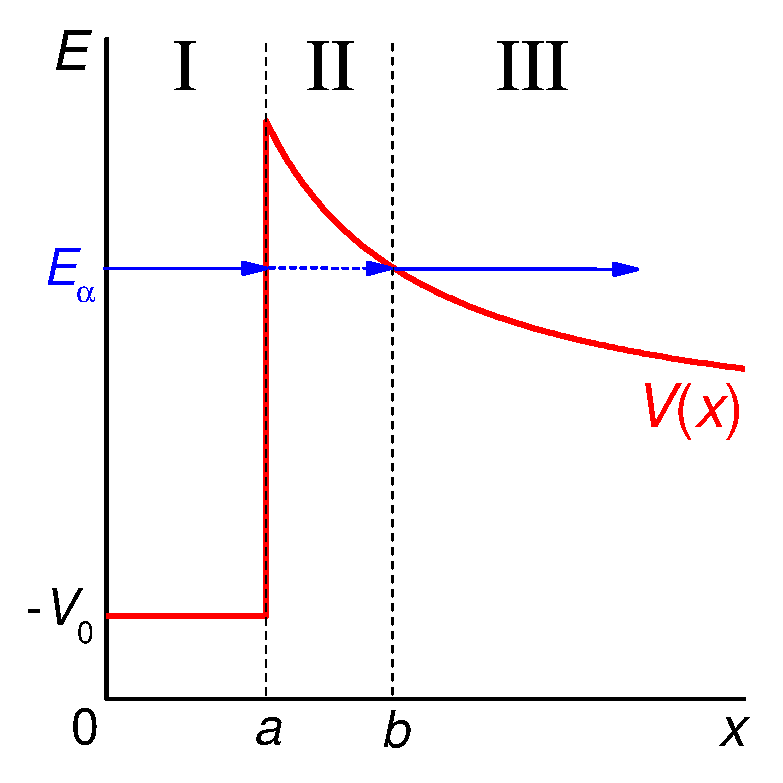
\epsfig{file=decay.eps,width=0.45\linewidth,keepaspectratio}
		\caption{
			Tunelování $\alpha$ částice o energii $E_{\alpha}$ z jádra přes Coulombickou bariéru.
		}
		\label{fig:AlphaDecay}
	\end{figure}	

	\begin{enumerate}
		\item 
			Ve WKB přiblížení odvoďte tzv. \emph{Gammovův koeficient průchodu}\index{koeficient průchodu!Gammovův}
			\begin{equation}
				\label{eq:Gammov}
				\important{
					T=\exp\left[-{\frac{2}{\hbar}}\int_{a}^{b}\abs{p(x)}\d x\right]
				},
			\end{equation}
			kde $\abs{p(x)}$ je absolutní hodnota \uv{hybnosti} částice v klasicky nedostupné oblasti vymezené body $a$, $b$, které ohraničují bariéru.
		
		\item				
			Nalezněte $T$ pro uvažovaný model $\alpha$ rozpadu.
		
		\item
			Střední dobu života lze aproximovat vztahem $\tau=\frac{1}{P_{\alpha}RT}$, kde $P_{\alpha}$ je pravděpodobnost,
			že se v jádře vydělí $\alpha$ částice (budeme předpokládat, že tato pravděpodobnost bude
			pro uvažovaná jádra $\approx1$) a $R$ je počet \uv{nárazů} $\alpha$ částice na bariéru za sekundu.
			Odhadněte $R$ a spočítejte $\tau$ a poločas rozpadu $T_{1/2}$.
		
		Pro poloměr atomu použijte přibližný vztah $a=a_{0}\sqrt[3]{A}$, kde $A$ je atomové číslo a $a_{0}\doteq1,\!2$ fm.
		
		\item
			Porovnejte číselně s hodnotami tří izotopů s poločasy rozpadu
			
			\begin{center}
				\begin{tabular}{|c|c|c|}
					\hline
					izotop & E (MeV) & $T_{1/2}$\\
					\hline
					\hline
					$^{144}_{\ 60}{\text{Nd}}$ & $1.8$ & $2\cdot10^{15}$ let\\
					\hline
					$^{224}_{\ 88}{\text{Ra}}$ & $5.7$ & $3.6$ dne\\
					\hline
					$^{212}_{\ 84}{\text{Po}}$ & $8.8$ & $0.3\,\mu$s\\
					\hline
				\end{tabular}
			\end{center}
		
		\item
			Určete de Broglieovy vlnové délky $\alpha$ částic v jádrech z tabulky a porovnejte je s rozměry jádra.
			Je WKB aproximace oprávněná?
		
	\end{enumerate}
	
\begin{solution}
	\begin{enumerate}
	\item
		Proces tunelování se rozdělí na tři oblasti:
		\begin{itemize}
		\item
			Oblast I: $x<a$, $E>V(x)$, vnitřek jádra.
		\item
			Oblast II: $a<x<b$, $E<V(x)$, Coulombická bariéra.
		\item
			Oblast III: $b<x$, $E>V(x)$, oblast vně jádra.
		\end{itemize}
		
		V oblasti III vně jádra je nenulová jen ta část vlnové funkce, která odpovídá prošlé částici vzdalující se od atomu,
		\begin{align}
			\psi_{\mathrm{III}}(x)
				&=\frac{C}{\sqrt{\abs{p(x)}}}\e^{\frac{\im}{\hbar}\int_{b}^{x}\abs{p(x')}\d x'+\im\frac{\pi}{4}}
				 =\lambda\e^{\im\left(I_{b}^{x}+\frac{\pi}{4}\right)}\nonumber\\
				&=\lambda\cos{\left[I_{b}^{x}+\frac{\pi}{4}\right]}+\im\lambda\sin{\left[I_{b}^{x}+\frac{\pi}{4}\right]},
		\end{align}
		kde je využito značení~\eqref{eq:WKBNotation}. 
		Do výrazu byla navíc přidána fáze $\pi/4$, což usnadní následné navazování vlnové funkce.
		Vlnová funkce v oblasti II se určí pomocí navazovacích vztahů~\eqref{eq:WKBConnectionDown1}---\eqref{eq:WKBConnectionDown2},
		\begin{equation}
			\psi_{\mathrm{II}}(x)=\lambda\e^{I_{x}^{b}}+\frac{\im}{2}\lambda\e^{-I_{x}^{b}}.
		\end{equation}
		
		Pomocí rozepsání integrálu
		\begin{align}
			\int_{x}^{b}&=\int_{a}^{b}-\int_{a}^{x} && \Longleftrightarrow & I_{x}^{b}&=I_{a}^{b}-I_{a}^{x}
		\end{align}
		a zkráceného označení
		\begin{equation}
			F\equiv\e^{-I_{a}^{b}}=\e^{-\frac{1}{\hbar}\int_{a}^{b}\abs{p(x)}\d x},
		\end{equation}
		vlnová funkce přejde do tvaru
		\begin{equation}
			\psi_{\mathrm{II}}(x)=\frac{\lambda}{F}\e^{-I_{a}^{x}}+\frac{\im}{2}\lambda F\e^{I_{a}^{x}}.
		\end{equation}
		Do oblasti I se následně naváže pomocí sešívacích podmínek~\eqref{eq:WKBConnectionUp1}---\eqref{eq:WKBConnectionUp2}:
		\begin{align}
			\psi_{\mathrm{I}}(x)
				&=\frac{2\lambda}{F}\sin\left[I_{a}^{x}+\frac{\pi}{4}\right]+\frac{\im}{2}\lambda F\cos\left[I_{a}^{x}+\frac{\pi}{4}\right]\nonumber\\										
				&=\underbrace{-C\left(\frac{1}{F}-\frac{F}{4}\right)\e^{\im\frac{\pi}{4}}}_{A}\frac{1}{\sqrt{\abs{p(x)}}}\e^{\im I_{x}^{a}}
					+\underbrace{\im C\left(\frac{1}{F}+\frac{F}{4}\right)\e^{-\im\frac{\pi}{4}}}_{B}\frac{1}{\sqrt{\abs{p(x)}}}\e^{-\im I_{x}^{a}}.						
		\end{align}
		Transmisní koeficient tedy vychází
		\begin{equation}
			T=\abs{\frac{C}{A}}^{2}=\frac{1}{\left(\frac{1}{F}-\frac{F}{4}\right)^{2}}\approx F^{2}\,,
		\end{equation}
		přičemž poslední rovnost platí za předpokladu $F\ll1$, což musí být splněno, aby bylo vůbec možné pro tento typ úlohy WKB aproximaci použít.
		Dosazení za $F$ dá hledaný Gammovův faktor~\eqref{eq:Gammov}.
		
	\item
		Do právě odvozeného Gammova vztahu pro pravděpodobnost průniku bariérou dosadíme potenciál~\eqref{eq:AlphaDecayPotential}.
		Klasická hybnost $\alpha$ částice o energii $E_{\alpha}$ v oblasti Coulombické části potenciálu je
		\begin{equation}
			p(x)=\sqrt{2M\left(E_{\alpha}-\frac{Z_{\alpha}Z\gamma}{x}\right)}.
		\end{equation}
		První bod obratu $a$ odpovídá poloměru jádra, druhý bod obratu se vypočítá z rovnice
		\begin{align}
			\label{eq:AlphaDecayTurningPoint}
			V(x)&=E_{\alpha} && \Longrightarrow & b&=\frac{Z_{\alpha}Z\gamma}{E_{\alpha}}\,,
		\end{align}
		takže
		\begin{align}
			I_{a}^{b}=\frac{1}{\hbar}\int_{a}^{b}\abs{p(x)}\d x
				&=\frac{\sqrt{2ME_{\alpha}}}{\hbar}\int_{a}^{b}\sqrt{\frac{Z_{\alpha}Z\gamma}{E_{\alpha}x}-1}\,\d x=\equationcomment{u=\frac{x}{b} \\ \d x=b\,\d u}\nonumber\\
				&=\underbrace{\frac{Z_{\alpha}Z\gamma}{\hbar}\sqrt{\frac{2M}{E_{\alpha}}}}_{\kappa}\int_{x=a}^{x=b}\sqrt{\frac{1}{u}-1}\,\d u=\equationcomment{u=y^{2} \\ \d u=2y\d y}\nonumber\\				
				&=2\kappa\int_{x=a}^{x=b}\sqrt{1-y^{2}}\,\d y,
		\end{align}
		což je tentýž integrál jako u WKB řešení harmonického oscilátoru~\eqref{eq:intsqrt} s primitivní funkcí
		\begin{align}
			I_{a}^{b}
				&=\kappa\left[y\sqrt{1-y^{2}}+\arcsin{y}\right]_{x=a}^{y=b}\nonumber\\
				&=\kappa\left[\sqrt{u}\sqrt{1-u}+\arcsin{\sqrt{u}}\right]_{u=\frac{a}{b}}^{1}=\nonumber\\
				&=\kappa\left[\arccos{\sqrt{\frac{a}{b}}}-\sqrt{\frac{a}{b}\left(1-\frac{a}{b}\right)}\right].
		\end{align}
		Pravděpodobnost průniku tedy vychází
		\begin{equation}
			T=\exp{\left\{\frac{2Z_{\alpha}Z\gamma}{\hbar}\sqrt{\frac{2M}{E_{\alpha}}}\left[\arccos{\sqrt{\frac{a}{b}}}-\sqrt{\frac{a}{b}\left(1-\frac{a}{b}\right)}\right]\right\}}
		\end{equation}
		kde $b$ je dáno vzorcem~\eqref{eq:AlphaDecayTurningPoint} a $a$ je poloměr jádra spočtený pomocí vztahu uvedeného v zadání příkladu.
		
	\item
		Počet \uv{nárazů} $\alpha$ částice na bariéru se odhadne jako
		\begin{equation}
			R=\frac{v_{\alpha}}{2a},
		\end{equation}
		kde $v_{\alpha}$ je rychlost $\alpha$ částice v jádře.
		Tu určíme z kinetické energie.
		Stačí počítat pomocí nerelativistických vztahů, protože rychlost vylétávajících $\alpha$ částic je malá ve srovnání s rychlostí světla, jak se lze přesvědčit z tabulky níže:
		\begin{equation}
			E_{\alpha}=v_{\alpha}^{2}/2M,
		\end{equation}
		přičemž energie je dána jako rozdíl klidové hmotnosti $M_{{}^{A}_{Z}X}$ jádra vstupujícího do reakce a klidové hmotnosti produktů (jádro $M_{{}^{A-4}_{Z-2}Y}$ + jádro helia $M_{{}^{4}_{2}\mathrm{He}}$)
		\begin{equation}
			E_{\alpha}=\frac{1}{c^{2}}\left(M_{{}^{A}_{Z}X}-M_{{}^{A-4}_{Z-2}Y}-M_{{}^{4}_{2}\mathrm{He}}\right)\,.
		\end{equation}
		Rychlost tedy vychází
		\begin{equation}
			v_{\alpha}=\sqrt{\frac{2\left(E_{\alpha}+V_{0}\right)}{M}}
		\end{equation}
		a z ní střední doba života
		\begin{equation}
			\tau=\frac{2a}{T}\sqrt{\frac{M}{2\left(E_{\alpha}+V_{0}\right)}}.
		\end{equation}
		Poločas rozpadu je $T_{1/2}=\tau\ln2$.

	\item
		Výsledky pro zadané izotopy jsou v následující tabulce:
		\begin{center}
			\begin{tabular}{|c|c|c|c|c|c|c|c|c|c|}
				\hline
				izotop & $\begin{array}{c}E_{\alpha} \\ \text{(MeV)}\end{array}$ & $\begin{array}{c}a \\ \text{(fm)}\end{array}$ & $\begin{array}{c}b \\ \text{(fm)}\end{array}$ 
				& $\frac{v_{\alpha}}{c}$ & $I_{a}^{b}$ & T & $\begin{array}{c}T_{1/2} \\ (s)\end{array}$ & $T_{1/2}$ \\
				\hline
				\hline
				$^{144}_{\ 60}{\text{Nd}}$ & $1.8$ & $6.3$ & $96$ & $0.17$ & $120$ & $7.2\cdot10^{-53}$ & $2.4\cdot10^{30}$ & $7.6\cdot10^{22}$ let \\
				\hline
				$^{224}_{\ 88}{\text{Ra}}$ & $5.7$ & $7.3$ & $45$ & $0.17$ & $73$ & $2.3\cdot10^{-32}$ & $8.5\cdot10^{9}$ & $98000$ dní \\
				\hline
				$^{212}_{\ 84}{\text{Po}}$ & $8.8$ & $7.2$ & $28$ & $0.18$ & $43$ & $3.1\cdot10^{-19}$ & $5.9\cdot10^{-4}$ & $590$ $\mu$s\\
				\hline
			\end{tabular}
		\end{center}
		Tento velmi zjednodušený výpočet tedy dává o několik řádů delší poločasy rozpadu, než jsou naměřené hodnoty ze zadání příkladu.
		Mnohem lepší shody se dosáhne, pokud se uvažuje $a_{0}=1.6$ fm, což v sobě může zahrnout difuzivitu jaderného povrchu.
		
	\item
		De Broglieovy vlnové délky $\alpha$ částic jsou
		\begin{equation}
			\lambda_{\alpha}=\frac{p_{\alpha}}{\hbar}=\frac{Mv_{\alpha}}{\hbar}\,.
		\end{equation}
		Číselně
		\begin{center}
			\begin{tabular}{|c|c|}
				\hline
				izotop & $\lambda_{\alpha}$ (fm) \\
				\hline
				\hline
				$^{144}_{\ 60}{\text{Nd}}$ & $0.32$ \\
				\hline
				$^{224}_{\ 88}{\text{Ra}}$ & $0.31$ \\
				\hline
				$^{212}_{\ 84}{\text{Po}}$ & $0.30$ \\
				\hline
			\end{tabular}
		\end{center}
		tedy asi 40 krát menší než je rozměr jádra.				
	\end{enumerate}

	\begin{note}
		Pro $a\ll b$ lze aproximovat
		\begin{equation}
			\arccos{\sqrt{\frac{a}{b}}}-\sqrt{\frac{a}{b}-\frac{a^{2}}{b^{2}}}\approx\frac{\pi}{2}-\sqrt{\frac{a}{b}}-\sqrt{\frac{a}{b}}=\frac{\pi}{2}-2\sqrt{\frac{a}{b}}\,.
		\end{equation}
		Pak
		\begin{align}
			\ln\tau
				&=\ln{\frac{2a}{v_{\alpha}}}+2I_{a}^{b}\nonumber\\
				&=\ln{\frac{2a_{0}\sqrt[3]{A}}{\sqrt{2\left(E_{\alpha}+V_{0}\right){M}}}}
					+\frac{2Z_{\alpha}Z\gamma}{\hbar}\sqrt{\frac{2M}{E_{\alpha}}}\left[\frac{\pi}{2}-2\sqrt{\frac{a_{0}}{Z_{\alpha}\gamma}}\sqrt{E_{\alpha}}A^{\frac{1}{6}}Z^{-\frac{1}{2}}\right]
		\end{align}
		a pro těžká jádra, pro která platí $A\approx 2Z$, dostaneme
		\begin{align}
			\ln\tau&=\frac{1}{3}\ln{Z}+\frac{1}{3}\ln{2}+\ln{\frac{2a_{0}}{\sqrt{\frac{2\left(E_{\alpha}-V_{0}\right)}{M}}}}+\frac{2Z_{\alpha}\gamma\sqrt{2M}}{\hbar}\frac{\pi}{2}\frac{Z}{\sqrt{E}}
				-4\frac{\sqrt{2Z_{\alpha}\gamma a_{0}M}}{\hbar}\sqrt[6]{2}Z^{\frac{2}{3}}
		\end{align}
		To je v souladu s experimentálně pozorovanou závislostí
		\begin{equation}
			(\ln{\tau})_{\mathrm{exp}}=C_{1}\left(\frac{Z}{\sqrt{E_{\alpha}}}-Z^{\frac{2}{3}}\right)-C_{2}\,.
		\end{equation}
	\end{note}
\end{solution}
	
\subsection{Dvojitá symetrická jáma}
	\begin{figure}[!htbp]
	\centering
	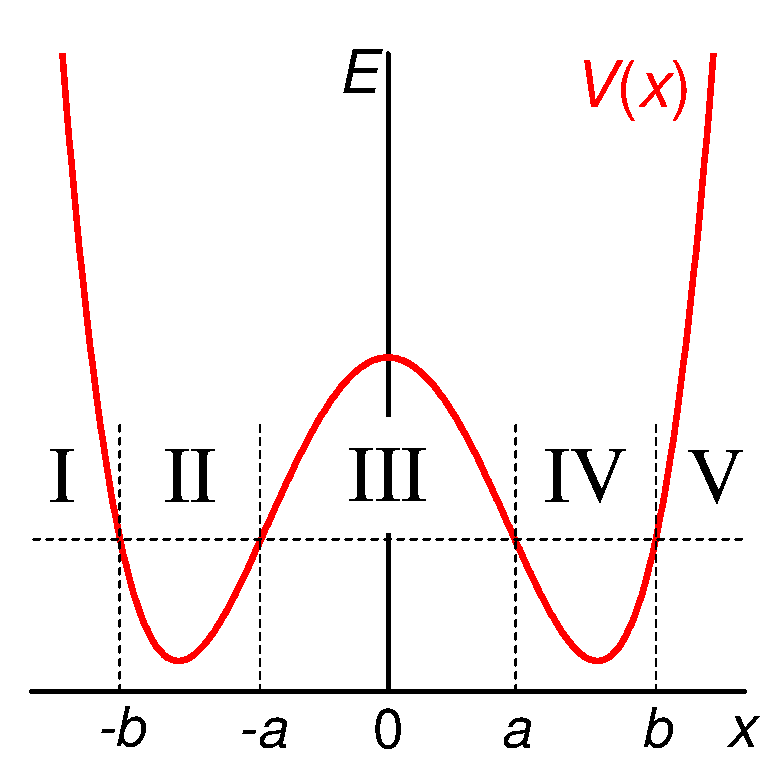
\epsfig{file=figures/dw.eps,width=0.5\linewidth,keepaspectratio}
	\caption{
		Potenciál dvojité symetrické jámy.
	}
	\label{fig:DoubleWell}
	\end{figure}	

	Částice o hmotnosti $M$ se pohybuje v sudém dvoujámovém potenciálu $V(x)=V(-x)$, viz obrázek~\ref{fig:DoubleWell}.
	Kdyby byly obě jámy oddělené nekonečně vysokou bariérou, 
	všechny energetické hladiny by byly dvakrát degenerované a odpovídající vlnové funkce by byly sudé a liché.
	Důsledkem nenulové pravděpodobnosti tunelování přes bariéru, která je v obrázku označena jako oblast III, 
	však dojde k interakci mezi hladinami a rozštěpení těchto degenerovaných dubletů.	
	\begin{enumerate}
	\item
		Nalezněte vztah pro vzdálenost $\Delta E$ mezi hladinami v dubletu pro obecný symetrický dvoujámový potenciál.
		
	\item
		Určete tuto vzdálenost pro speciální potenciál ve tvaru
		\begin{equation}
			\label{eq:DoubleWellPotential}
			V(x)=\frac{g^{2}}{8}\left(x^{2}-x_{0}^{2}\right)^{2},
		\end{equation}
		kde $x_{0}$ určuje $x$-ové souřadnice minim, $g$ je konstanta.
		Předpokládejte, že energie je dostatečně hluboko v jamách, kde lze potenciál $V(x)$ aproximovat potenciálem harmonického oscilátoru.
	
	\item
		Srovnejte číselně s výsledkem úkolu ze 3. cvičení zimního semestru.	
	\end{enumerate}

\begin{solution}
	\begin{enumerate}
	\item
		Tunelující systém se rozdělí na pět oblastí podle obrázku~\ref{fig:DoubleWell}.
		Všechny výpočty budou ve zkrácené notaci~\eqref{eq:WKBNotation}.
		Využívat se budou navazovací podmínky~\eqref{eq:WKBConnectionDown1}---\eqref{eq:WKBConnectionUp2}.
		
		\begin{itemize}
		\item
			V oblasti I musí vlnová funkce exponenciálně ubývat pro $x\rightarrow-\infty$, takže
			\begin{equation}
				\psi_{\mathrm{I}}(x)=\frac{C}{\sqrt{\abs{p(x)}}}\e^{-\frac{1}{\hbar}\int_{x}^{-b}\abs{p(x')}\d x'}=\lambda\e^{-I_{x}^{-b}}.
			\end{equation}
			
		\item
			Do oblasti II se vlnovou funkci napojí pomocí vztahů~\eqref{eq:WKBConnectionDown1}---\eqref{eq:WKBConnectionDown2}:
			\begin{equation}
				\psi_{\mathrm{II}}(x)=2\lambda\sin{\left[I_{-b}^{x}+\frac{\pi}{4}\right]}.
			\end{equation}
			Vlnovou funkci je nyní potřeba upravit do takové formy, aby bylo možné pro navázání do oblasti III použít vztahů~\eqref{eq:WKBConnectionUp1}---\eqref{eq:WKBConnectionUp2}:
			\begin{align}
				\psi_{\mathrm{II}}(x)
					&=2\lambda\underbrace{\sin{\left[I_{-b}^{-a}-I_{x}^{-a}+\frac{\pi}{4}\right]}}_{\sin{(a+b)}=\sin{a}\cos{b}+\cos{a}\sin{b}}\nonumber\\
					&=2\lambda\left\{\underbrace{\sin{I_{-b}^{-a}}}_{S}\cos\left[-I_{x}^{-a}+\frac{\pi}{4}\right]+\underbrace{\cos{I_{-b}^{-a}}}_{C}\sin\left[-\int_{x}^{-a}+\frac{\pi}{4}\right]\right\}
			\end{align}
			Je nutné ošetřit i znaménko $-$ před integrály v argumentech sinu a cosinu.
			K tomu se využijí vztahy
			\begin{align}
				\cos\left[-I+\frac{\pi}{4}\right]
					&\stackrel{\cos\text{ sudá}}{=}\cos\left[I-\frac{\pi}{4}\right]=\underbrace{\cos\left[I+\frac{\pi}{4}-\frac{\pi}{2}\right]}_{\cos{(a+b)}=\cos{a}\cos{b}-\sin{a}\sin{b}}\nonumber\\
					&=\cos\left[I+\frac{\pi}{4}\right]\underbrace{\cos\left(-\frac{\pi}{2}\right)}_{0}-\sin\left[I+\frac{\pi}{4}\right]\underbrace{\sin\left(-\frac{\pi}{2}\right)}_{-1}\nonumber\\
					&=\sin\left[I+\frac{\pi}{4}\right]\,,
			\end{align}
			a analogicky
			\begin{equation}
				\sin\left[-I+\frac{\pi}{4}\right]=\cos\left[I+\frac{\pi}{4}\right].
			\end{equation}
			Vlnovou funkci v oblasti II lze tedy zapsat ve tvaru
			\begin{equation}
				\psi_{\mathrm{II}}(x)=2\lambda\left\{S\sin\left[I_{x}^{-a}+\frac{\pi}{4}\right]+C\cos\left[I_{x}^{-a}+\frac{\pi}{4}\right]\right\}.
			\end{equation}
		
		\item
			Do oblasti III se posuneme za pomoci sešívacích vztahů~\eqref{eq:WKBConnectionUp1}---\eqref{eq:WKBConnectionUp2} a vlnovou funkci ihned upravíme pro navázání do následující oblasti IV:
			\begin{align}
				\psi_{\mathrm{III}}(x)
					&=\lambda S\e^{-I_{-a}^{x}}+2\lambda C\e^{I_{-a}^{x}}\nonumber\\
					&=\lambda S\underbrace{\e^{-I_{-a}^{a}}}_{F}\e^{I_{x}^{a}}+2\lambda C\e^{I_{-a}^{a}}\e^{-I_{x}^{a}}\nonumber\\
					&=\lambda SF\e^{I_{x}^{a}}+\frac{2\lambda C}{F}\e^{-I_{x}^{a}}
			\end{align}
			
		\item
			V navazování se pokračuje dále do oblasti IV pomocí vztahů~\eqref{eq:WKBConnectionDown1}---\eqref{eq:WKBConnectionDown2}:
			\begin{align}
				\psi_{\mathrm{IV}}(x)
					&=\lambda SF\cos\left[I_{a}^{x}+\frac{\pi}{4}\right]+\frac{4\lambda C}{F}\sin\left[I_{a}^{x}+\frac{\pi}{4}\right]\nonumber\\
					&=\lambda SF\cos\left[I_{a}^{b}-I_{x}^{b}+\frac{\pi}{4}\right]+\frac{4\lambda C}{F}\sin\left[I_{a}^{b}-I_{x}^{b}+\frac{\pi}{4}\right]\nonumber\\
					&=\lambda SF\left\{C\sin\left[I_{x}^{b}+\frac{\pi}{4}\right]-S\cos\left[I_{x}^{b}+\frac{\pi}{4}\right]\right\}\nonumber\\
					&\qquad+\frac{4\lambda C}{F}\left\{S\sin\left[I_{x}^{b}+\frac{\pi}{4}\right]+C\cos\left[I_{x}^{b}+\frac{\pi}{4}\right]\right\}\nonumber\\
					&=\lambda SC\left(F+\frac{4}{F}\right)\sin\left[I_{x}^{b}+\frac{\pi}{4}\right]+\lambda\left(-S^{2}F+\frac{4C^{2}}{F}\right)\cos\left[I_{x}^{b}+\frac{\pi}{4}\right].
			\end{align}
			Využívá se zde sudosti potenciálu, díky níž
			\begin{align}
				V(x)&=V(-x) && \Longrightarrow & p(x)&=p(-x) && \Longrightarrow & I_{-b}^{-a}&=I_{a}^{b}.
			\end{align}
			
		\item
			Poslední navazování do oblasti V se provedeme opět pomocí vztahů~\eqref{eq:WKBConnectionUp1}---\eqref{eq:WKBConnectionUp2}:
			\begin{equation}
				\psi_{\mathrm{V}}(x)=\frac{\lambda SC}{2}\left(F+\frac{4}{F}\right)\e^{-I_{b}^{x}}+\underbrace{\lambda\left(-S^{2}F+\frac{4C^{2}}{F}\right)}_{Z}\e^{I_{b}^{x}}
			\end{equation}		
		\end{itemize}
	
		Celková vlnová funkce musí být normovatelná (kvadraticky integrovatelná), tj. nesmí divergovat  pro $x\rightarrow\infty$.
		Musí být tedy splněno $Z=0$, tj.
		\begin{align}
			\lambda\left(-S^{2}F+\frac{4C^{2}}{F}\right)&=0\nonumber\\
			S^{2}&=\frac{4C^{2}}{F^{2}}\nonumber\\
			\frac{C}{S}&=\pm\frac{1}{2}F
		\end{align}
		To po dosazení za $S$, $C$ a $F$ vede na rovnici
		\begin{align}
			\cotg{\frac{1}{\hbar}\int_{a}^{b}p(x)\d x}=\pm\frac{1}{2}\e^{-\frac{1}{\hbar}\int_{-a}^{a}\abs{p(x)}\d x}.
		\end{align}
		
		Následovat bude několik aproximací. 
		Předně budeme předpokládat, že prostupnost bariéry III je malá, takže $F\approx0$ a lze psát
		\begin{equation}
			\pm\frac{1}{2}F\approx\cotg{\left[\mp\frac{1}{2}F+\pi\left(n+\frac{1}{2}\right)\right]},
		\end{equation}
		kde $n\in\mathbb{N}_{0}$.
		To vede k rovnici (kvantovací podmínce)
		\begin{equation}
			\label{eq:DoubleWellE}
			\frac{1}{\hbar}\int_{a}^{b}p(x)\d x=\pi\left(n+\frac{1}{2}\right)\pm\frac{1}{2}\e^{-\frac{1}{\hbar}\int_{-a}^{a}\abs{p(x)}\d x}
		\end{equation}
	
		Kdyby nebylo tunelování mezi dvěma jamami, spektrum $E_{n}^{(0)}$ by na základě Bohrova-Sommerfeldova kvantování~\eqref{eq:BohrSommerfeld} bylo dáno rovnicí
		\begin{equation}
			\int_{a}^{b}\sqrt{2M\left[E_{n}^{(0)}-V(x)\right]}\,\d x=\pi\hbar\left(n+\frac{1}{2}\right).
		\end{equation}
		Ve skutečnosti však dochází k tunelování a spektrum je dáno rovnicí~\eqref{eq:DoubleWellE}.
		Označme
		\begin{equation}
			E_{n}=E_{n}^{(0)}+\epsilon.
		\end{equation}
		a rozviňme levou stranu rovnice~\eqref{eq:DoubleWellE} okolo $E_{n}^{(0)}$:
		\begin{align}
			\frac{1}{\hbar}\int_{a}^{b}\underbrace{\sqrt{2M\left[E_{n}-V(x)\right]}}_{p(x;E_{n})}\,\d x
				&=\frac{1}{\hbar}\int_{a}^{b}p(x;E_{n}^{(0)})\d x+\frac{\epsilon}{\hbar}\int_{a}^{b}\partialderivative{p}{E}(x;E_{n}^{(0)})\d x+\dotsb\nonumber\\
				&\approx\pi\left(n+\frac{1}{2}\right)+\frac{\epsilon}{\hbar}\underbrace{2M\int_{a}^{b}\frac{\d x}{\sqrt{2M\left[E_{n}^{(0)}-V(x)\right]}}}_{\int_{a}^{b}\frac{\d x}{v(x)}=\frac{1}{2}\oint\frac{\d x}{v(x)}=\frac{T}{2}}\,,
		\end{align}
		kde $T$ odpovídá periodě klasické trajektorie na energii $E_{n}^{(0)}$ (úhlová frekvence je $\Omega=2\pi/T$).
		Dosazení do~\eqref{eq:DoubleWellE} vede k jednoduchému vztahu
		\begin{equation}
			\epsilon=\pm\frac{\hbar\Omega}{2\pi}E
		\end{equation}
		z něhož lze určit rozštěpení hladin jako
		\begin{equation}
			\label{eq:DoubleWellSplit}
			\important{\Delta E_{n}=\frac{\hbar\Omega}{\pi}\e^{-\frac{1}{\hbar}\int_{-a}^{a}\abs{p(x)}\d x}}.
		\end{equation}
	
	\item
		Za předpokladu, že se částice nachází na energii dostatečně blízko dnu jámy, lze potenciál~\eqref{eq:DoubleWellPotential} rozvinout okolo $x_{0}$:
		\begin{align}
			V(x)
				&=\frac{g^{2}}{8}\left(x+x_{0}\right)^{2}{\underbrace{\left(x-x_{0}\right)}_{y}}^{2}=\frac{g^{2}}{8}\left(y+2x_{0}\right)^{2}y^{2}\nonumber\\
				&\approx\frac{1}{2}g^{2}x_{0}^{2}y^{2}=\frac{1}{2}M\Omega^{2}y^{2}\,,
		\end{align}
		takže pohyb hluboko v jámě přibližně odpovídá periodickému pohybu harmonického oscilátoru s frekvencí
		\begin{equation}
			\Omega=\frac{gx_{0}}{\sqrt{M}}
		\end{equation}
		a spektrem
		\begin{equation}
			E_{n}=\hbar\Omega\left(n+\frac{1}{2}\right).
		\end{equation}
		Body obratu (řešení rovnice $V(x)=E_{n}$) pak jsou
		\begin{equation}
			\begin{array}{c}a \\ b\end{array}=x_{0}\mp\sqrt{\frac{\hbar}{M\Omega}\left(n+\frac{1}{2}\right)}
		\end{equation}
		a speciálně pro základní stav $n=0$
		\begin{subequations}	
			\begin{align}
				a&=x_{0}-\sqrt{\frac{\hbar}{M\Omega}},\\ 
				b&=x_{0}+\sqrt{\frac{\hbar}{M\Omega}}.
			\end{align}
		\end{subequations}
			
		Integrál z kvantovací podmínky~\eqref{eq:DoubleWellE} je
		\begin{align}
			\hbar I_{-a}^{a}
				&=2\hbar I_{0}^{a}=2\int_{0}^{a}\sqrt{2M\left[\frac{g^{2}}{8}\left(x_{0}^{2}-x^{2}\right)^{2}-\frac{1}{2}\hbar\Omega\right]}\,\d x\nonumber\\
				&=\int_{0}^{a}\underbrace{g}_{\frac{\Omega}{x_{0}}\sqrt{M}}\sqrt{M}\left(x_{0}^{2}-x^{2}\right)\sqrt{1-\frac{4\hbar\Omega}{g^{2}\left(x_{0}^{2}-x^{2}\right)^{2}}}\,\d x\nonumber\\
				&\approx\int_{0}^{a}\frac{M\Omega\left(x_{0}^{2}-x^{2}\right)}{x_{0}}\d x-2\int_{0}^{a}\frac{\hbar x_{0}}{x_{0}^{2}-x^{2}}\d x\nonumber\\
				&=\int_{0}^{a}\left[M\Omega x_{0}^{2}-\frac{M\Omega x^{2}}{x_{0}}-\frac{\hbar}{x_{0}-x}-\frac{\hbar}{x_{0}+x}\right]\d x\nonumber\\
				&=\left[M\Omega x_{0}^{2}x-\frac{M\Omega x^{3}}{3x_{0}}+\hbar\ln\left(x_{0}-x\right)-\hbar\ln\left(x_{0}+x\right)\right]_{0}^{a}\nonumber\\
				&=M\Omega x_{0}\left(x_{0}-\sqrt{\frac{\hbar}{M\Omega}}\right)
					-\underbrace{\frac{M\Omega}{3x_{0}}\left(x_{0}-\sqrt{\frac{\hbar}{M\Omega}}\right)^{3}}_{\approx\frac{M\Omega x_{0}^{2}}{3}\left(1-\frac{3}{x_{0}}\sqrt{\frac{\hbar}{M\Omega}}+\frac{3}{x_{0}^{2}}\frac{\hbar}{M\Omega}\right)}
					+\underbrace{\hbar\ln{\sqrt{\frac{\hbar}{M\Omega}}}}_{\hbar\ln{x_{0}}+\hbar\ln{\frac{1}{x_{0}}\sqrt{\frac{\hbar}{M\Omega}}}}\nonumber\\
				&\qquad-\underbrace{\hbar\ln{\left(2x_{0}-\sqrt{\frac{\hbar}{M\Omega}}\right)}}_{\hbar\ln{x_{0}}+\hbar\ln\left(2-\frac{1}{x_{0}}\sqrt{\frac{\hbar}{M\Omega}}\right)}\nonumber\\
				&\approx\frac{2M\Omega x_{0}^{2}}{3}-\hbar+\hbar\ln\sqrt{\frac{\hbar}{4M\Omega x_{0}^{2}}}+\mathcal{O}\left(\hbar^{\frac{2}{3}}\right),
		\end{align}
		za předpokladu, že Planckova konstanta $\hbar$ je oproti ostatním veličinám malý parametr.
		
		Po dosazení do~\eqref{eq:DoubleWellSplit} vychází pro vzdálenost hladin v dubletech
		\begin{equation}
			\Delta E_{0}
				=\frac{\Omega\hbar}{\pi}\e^{-I_{-a}^{a}}\approx\frac{\Omega\hbar}{\pi}\sqrt{\frac{4M\Omega x_{0}^{2}}{\hbar}}\e^{-\frac{2M\Omega x_{0}^{2}}{3\hbar}+1}
				=\frac{2}{\pi}\sqrt{\frac{\hbar g^{3}x_{0}^{5}}{M}}\e^{-\frac{2\sqrt{M}g x_{0}^{3}}{3\hbar}+1}.
		\end{equation}
		Sbírka~\cite{Cini2012} uvádí výsledek odlišně
		\begin{equation}
			\Delta E_{0}'=2\sqrt{\frac{\hbar g^{3}x_{0}^{5}}{M}}\e^{-\frac{2\sqrt{M}g x_{0}^{3}}{3\hbar}}\,,
		\end{equation}
		a to i přesto, že integrál $I_{-a}^{a}$ v ní vychází stejně jako zde.
		Tento výraz $\Delta E_{0}'$ nicméně lépe souhlasí s přesnějšími metodami, viz např. následující bod.
			
	\item
		Dvoujámový potenciál, se kterým budeme nyní získaný výsledek srovnávat, má tvar
		\begin{equation}
			V(x)=-\frac{1}{2}x^{2}+x^{4}=\left(x^{2}-\frac{1}{4}\right)^{2}-\frac{1}{16},
		\end{equation}
		takže se jedná přibližně o potenciál~\eqref{eq:DoubleWellPotential} s
		\begin{equation}
			g=2\sqrt{2}\,,\qquad x_{0}=\frac{1}{2}
		\end{equation}
		a spektrum je posunuté o $\frac{1}{16}$ energetické jednotky dolů.
		
		Pro dostatečně malé hodnoty $\hbar$ (v úloze se počítalo s $\hbar=0.02$) dostaneme pro základní stav
		\begin{align}
			\Omega&=\frac{g x_{0}}{\sqrt{M}}=\sqrt{2}\approx1.4142\nonumber\\
			E_{0}&=\frac{1}{2}\hbar\Omega-\frac{1}{16}\approx-0.0484\nonumber\\
			\Delta E_{0}'&=1.81\cdot 10^{-6}
		\end{align}
		Naproti tomu na základě numerické diagonalizace jsme dostali
		\begin{align}
			E_{0}&=-0.0489 & \Delta E=1.86\cdot 10^{-6}.
		\end{align}
		Pro menší hodnoty $\hbar$ bychom dostali lepší shodu.						
	\end{enumerate}
\end{solution}
	

\subsection{Coulombické pole}	
    WKB metodu lze aplikovat také na problémy se sféricky symetrickým polem.
    Schrödingerova rovnice pro radiální část vlnové funkce $R(r)$ obecného sféricky symetrického problému má tvar
    \begin{equation}
        \frac{1}{r^{2}}\frac{\d}{\d r}r^{2}\frac{\d}{\d r}R(r)+\frac{2m}{\hbar^{2}}\left(E-V_{\ti{ef}}(r)\right)R(r)
            =0,
    \end{equation}
    kde 
    \begin{equation}
    V_{\ti{ef}}(r)
        \equiv V(r)+\frac{\hbar^{2}l(l+1)}{2mr^{2}}
    \end{equation}
    je efektivní potenciál, zahrnující v sobě centrifugální člen.
    
    Zavedením substituce $R(r)=u(r)/r$ dostaneme rovnici
    \begin{equation}
        \frac{\d^{2}}{\d r^{2}}u(r)+k^{2}(r)u(r)
            =0,
    \end{equation}
    kde $k^{2}(r)=2m/\hbar^{2}(E-V_{\ti{ef}})$.
    
    WKB metoda pro sféricky symetrické potenciály dává dobré výsledky jedině v případě, 
    aplikujeme-li tzv. \emph{Langerovu korekci}\index{korekce!Langerova}, která spočívá v nahrazení 
    \begin{equation}
        \important{l(l+1)\rightarrow(l+\frac{1}{2})^{2}}
    \end{equation}
    (dá se odvodit z asymptotiky vlnových funkcí; původní práce Rudolpha E. Langera je v~\cite{Langer1937}).
    Vázané stavy lze pak nalézt z rovnice ekvivalentní Bohrově-Sommerfeldově kvantovací podmínce
    \begin{equation}
        \int_{r_{1}}^{r_{2}}k'(r)\d r
            =\left(n_{\ti{r}}+\frac{1}{2}\right)\pi,
    \end{equation}
    přičemž $k'(r)$ zahrnuje Langerovu korekci, $n_{\ti{r}}=0,1,\dots$ je radiální kvantové číslo a
    $r_{1,2}$ jsou body obratu klasické trajektorie s hybností $p'(r)=\hbar k'(r)$.
    
    Uvažujte konkrétní případ pohybu částice v Coulombickém poli
    \begin{equation}
        V(r)=-\frac{\gamma}{r}.
    \end{equation}
    kde $\gamma=e^{2}/(4\pi\epsilon_{0})$.
    
    \begin{enumerate}
        \item 
            Nalezněte body obratu $r_{1,2}$ trajektorie s energií $E$ (počítejte s Langerovou korekcí).
        
        \item 
            Pomocí WKB přiblížení nalezněte spektrum, tj. stavy s energií $E<0$.
        
        \item
            Porovnejte toto spektrum se spektrem získaným přesným řešením Schrödingerovy rovnice.
    \end{enumerate}

    \begin{solution}
        Řešení formou hry naleznete na následujících odkazech:
        \href{http://pavelstransky.cz/cviceniktvt/WKBLanger_1.1_linux.zip}{Linux},
        \href{http://pavelstransky.cz/cviceniktvt/WKBLanger_1.1_windows.zip}{Windows}.
    \end{solution}

\subsection{Homogenní pole}
Částice o hmotnosti $M$ (hopík) skáče v homogenním (např. gravitačním) poli,
přičemž od podložky se odráží bez ztráty energie.
Potenciál se tedy dá vyjádřit jako
\begin{equation}
    V(z)=
    \begin{cases}
    mgz & z > 0 \\
    \infty & z < 0
    \end{cases}
\end{equation}

\begin{enumerate}
\item 
        Řešení pomocí WKB metody:
        \begin{itemize}
        \item 
            Nalezněte body obratu, má-li částice energii $E$.

        \item 
            Pomocí WKB přiblížení vypočítejte energetické spektrum.

        \item
            Nalezněte WKB vlnové funkce v klasicky dostupné i nedostupné oblasti.
            Vlnové funkce nemusíte normovat.
        \end{itemize}

    \item 
        Hledání základního stavu variační metodou:
        \begin{itemize}
        \item 
            Podle chování potenciálu navrhněte vhodnou testovací funkci s jedním parametrem (dodatečný parametr bude fixovat normalizaci).

        \item 
            Nalezněte optimální hodnotu parametru a jemu odpovídající přibližnou energii základního stavu.
        \end{itemize}

    \item 
        Srovnáním energií základního stavu získaných oběma metodami určete, která metoda dává základní stav přesněji.
\end{enumerate}	

